\section{Prior work}
\label{sec:prior_work}

%-------------------------------------------------------------------------
\subsection{Zero-Noise Extrapolation}
As discussed earlier, QEM methods rely on tractable increase in quantum resources along with additional classical processing.
Here we briefly describe zero-noise extrapolation \cite{PhysRevLett.119.180509,PhysRevX.7.021050} (ZNE) as a widely used method.
ZNE requires linear quantum runtime overhead combined with a classical extrapolation subroutine, making it atractive as a case agnaustic method.
To be more specific the ZNE approach is comprised of three steps: \textbf{(i)} Execute the target algorithm to obtain the scalar output,
\textbf{(ii)} execute theoretically equivalent versions of the algorithm but in a noisier setting, \textbf{(iii)} estimate the noiseless output by fitting a well-educated model.
These steps are showcased in Figure \ref{fig:zne} where noise amplification is achieved by global circuit folding, where the algorithm $U$ is uncomputed $U^\dagger$ and recomputed based on the unitary constraint
(see Appendix \ref{sec:computation}). This process effectively amplifies the noise while remaining theoretically equivalent to the original algorithm.

\begin{figure}
    \centering
    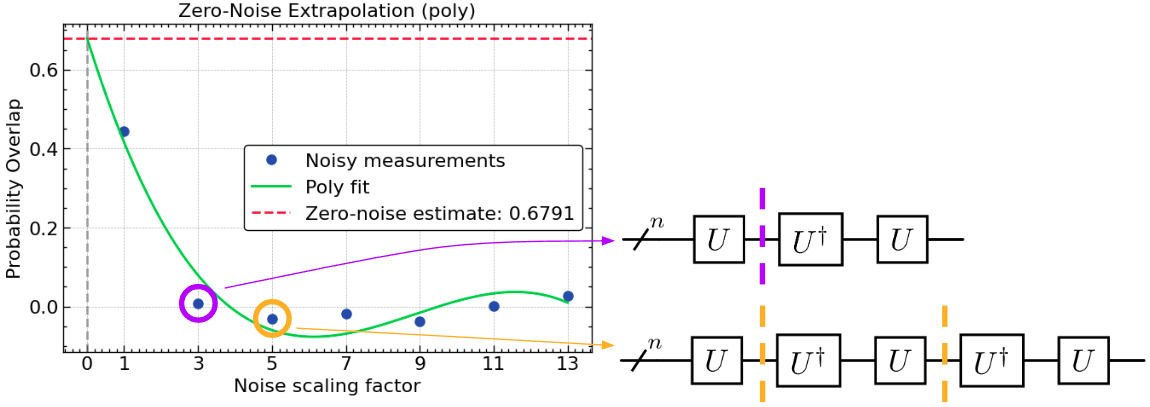
\includegraphics[width=\linewidth]{figures/zne.png}
    \caption{Error-mitigated estimate obtained using zero-noise extrapolation. Here extrapolation is performed using seven noisy data points.
    These are obtained by undoing $U^\dagger$ and redoing $U$ the quantum algorithm as many times as the scaling factor dectatets.}
    \label{fig:zne}
\end{figure}

Although ZNE is simple and powerful, it comes with some significant limitations. Firstly extrapolation is biased towards the rigid trend of the specified function, while it can be unstable when the noisy samples are similar.
Secondly granularity, noise drift.
It is also worth mentioning that using a neural network instead of function fitting is an active area of research.

%-------------------------------------------------------------------------
\subsection{The Neural Noise Accumulation Surrogate}
\label{sec:nnas-background}

Machine-learning approaches to quantum error mitigation (ML-QEM) typically treat the mapping from noisy to noiseless expectation values as an unstructured regression problem \cite{placidi2026deeplearningapproachesquantum}, learned from data produced by simulating or executing a circuit under a noise model. While such models can be effective at learning circuit features \cite{liao_machine_2024}, their black-box nature limits both their data efficiency and their ability to generalize across circuit depths.

The Neural Noise Accumulation Surrogate (NNAS) \cite{xu2025} addresses this by embedding a physical mechanisms directly into the network architecture. For a circuit of $L$ layers, NNAS models the noisy-to-noiseless mapping as a layer-wise sequential process, mirroring the way noise physically compounds as a circuit executes. Each noisy layer $\tilde{u}_l$ is decomposed via \emph{Maximum Noise Decomposition} (MND) into an ideal unitary $u_l$ composed with a stochastic, completely positive trace-preserving (CPTP) channel $\mathcal{E}_l$,
\begin{equation}
    \mathcal{E}_l = (1-p_l)\mathcal{I} + p_l \Lambda_l ,
\end{equation}
where $p_l$ is an empirically estimated effectiveness rate and $\Lambda_l$ is the residual CPTP channel (see also Appendix \ref{sec:errors}).
Propagating each layer's noise to the end of the circuit yields a cumulative noise envelope $R_l = \mathcal{U}_l \mathcal{N}_l \mathcal{U}_l^\dagger$, where $\mathcal{U}_l$ and $\mathcal{N}_l$ denote the circuit and noise channels respectively. The impact on the observable of interest is captured by a scalar impact factor $r_l$ via
\begin{equation}
    \text{Tr}[R_l\rho_l O] \rightarrow r_l\text{Tr}[\rho_l O]
\end{equation}
for a given target observable $O$.
As shown in \cite{xu2025} this yields the mitigated estimate
\begin{equation}
    y_l^{\mathrm{em}} = \frac{\tilde{y}_l}{\prod_{j=1}^{l}(1-\hat{p}_j) + \hat{r}_l} .
    \label{eq:mitigation}
\end{equation}
The first term in the denominator is a closed-form prior derived from the estimated effectiveness rates, the second term, $\hat{r}_l$, is the quantity NNAS is trained to predict. A schemantic representation of the autoregressive task is given by Figure \ref{fig:autoregressive_qem}.

\begin{figure}
    \centering
    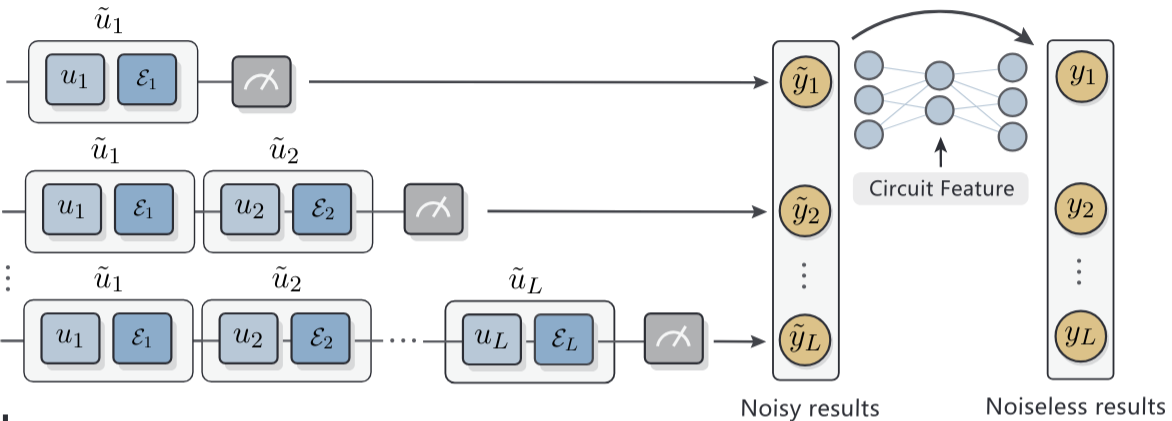
\includegraphics[width=\linewidth]{figures/autoregressive_qem.png}
    \caption{The illustration of layer-wise quantum sequential task. Figure adapted from \cite{xu2025}.}
    \label{fig:autoregressive_qem}
\end{figure}

Architecturally, NNAS instantiates this decomposition as a recurrent \emph{uniform neural accumulator}, a single hidden state $H_l$ updated as
\begin{equation}
    H_l = F(H_{l-1}, x_l),
\end{equation}
where $x_l$ embeds the circuit and device specification at layer $l$. This recursion mirrors the layer-by-layer composition of $\mathcal{U}_l$ and $\mathcal{N}_l$, so that $H_l$ implicitly represents the compressed state of noise accumulated up to layer $l$. Low-rank surrogates $\hat{\mathcal{U}}_l, \hat{\mathcal{N}}_l$ are recovered from $H_l$ via linear projections, and an attention mechanism,
\begin{equation}
    A_l = \mathrm{softmax}\!\left(\frac{\hat{\mathcal{U}}_l \hat{\mathcal{N}}_l^{T}}{\sqrt{d}}\right)\hat{\mathcal{U}}_l ,
\end{equation}
emulates the conjugate structure of $R_l = \mathcal{U}_l\mathcal{N}_l\mathcal{U}_l^\dagger$ before a final readout layer produces $\hat{r}_l$. Trained end-to-end against Eq.~\ref{eq:mitigation}, this design lets NNAS achieve strong mitigation accuracy from substantially less training data than unstructured regressors, and to degrade more slower with circuit depth, since the recurrent structure generalizes naturally to layer counts beyond those seen in training.

This efficiency, however, is inseparable from the specific physical assumption baked into the architecture: MND, and the effectiveness-rate prior it produces, is defined only for \emph{stochastic} CPTP channels. It has no representation for \emph{coherent} errors which act as unitary deviations rather than probabilistic mixtures. Such errors do not shrink the accumulated-noise prior $\prod_j(1-\hat p_j)$ toward zero in the way decoherence does. A single recurrent state $H_l$ trained under this architecture must therefore implicitly absorb both effects through the same update rule and the same scalar prior, with no structural signal distinguishing coherent noise.

In this work we extend the NNAS architecture by seperating the accumulation of noise into different branches for the two physically distinct error processes. A dedicated recurrent branch for coherent error accumulation is intriduced that is coupled to the existing stochastic branch and fused before the shared attention extractor.
